\section{Videojuego.}\label{Videojuego}
	En esta sección se define lo que es un videojuego, sus características, los tipos de 
	clasificaciones, haciendo principal inacpie en las dos de las más importantes: la
	 clasificación por su contenido y por su jugabilidad, finalizando con la el 
	 estado de la industria del videojuego a nivel internacional y en México.
	
	\subsection{¿Qué es un videojuego?}\label{Defvideojuego}
El grupo Carricay define al videojuego como: "una aplicación interactiva orientada
 al entretenimiento que, a través de ciertos mandos o controles, permite simular 
 experiencias en la pantalla de un televisor, una computadora u otro dispositivo 
 electrónico"\cite{Ref_DefVideo}.
	
	\subsection{Caracteristicas del videojuego.}\label{CaracVideojuego}
	Al igual que con otros productos tecnológicos, la evolución de los videojuegos 
	ha sido vertiginosa, resultando complicado mencionar características comunes 
	para todos los videojuegos. Sin embargo, en el libro “Marketing y videojuegos: 
	Product pacement, in-game, adevertising y advergaming” se menciona que existen seis 
	características comunes en los videojuegos: Interactividad, entretenimiento, 
	jugabilidad, simulación \textbackslash virtualidad, inmersión y multiplataformidad 
	\cite{RefCarac}; a continuación se hace menciona en que consisten cinco de las seis 
	características, esto debido a que la última no se encuentra presente en todos los 
	juegos y el mismo autor de la obra la menciona como una caracteristica opcional a 
	tomar en cuenta:
	%%para los autores mejor mencionar obra
	\begin{itemize}
		\item \textbf{Interactividad:} En el articulo "Defining Virtual Reality:
		 Dimensions Determining Telepresence" se define la interactividad como la 
		 capacidad de los usuarios para participar y modificar la forma y el contenido 
		 de un entorno mediado en tiempo real\cite{RefInteractividad}.  
		
		\item \textbf{Entretenimiento:} en el articulo "Las Tecnologías del
		 Entretenimiento: Pasado, Presente y Futuro", el entretenimiento "se asocia, 
		 usualmente, de hacer algo que nos divierte, algo que podemos hacer solos o con 
		 otros, para entretenernos o divertirnos, en nuestro tiempo libre, o tal vez, 
		 algo que nos relaje o que nos haga reír"\cite{RefEntretenimiento}. 
		
		\item \textbf{Jugabilidad:} en el libro “Marketing y videojuegos: 
	Product pacement, in-game, adevertising y advergaming” se define la jugabilidad 
	como "la relación que existe entre todas las acciones reacciones e interacciones
	 tanto del videojugador como el videojuego como entre los propios sistemas y 
	 subsistemas programados en el videojuego"\cite{RefCarac}.
		
		\item \textbf{Simulación \textbackslash Virtualidad:} La simulación "se trata 
		de una representación a medida cuyo objetivo nos permite interactuar y 
		relacionarnos con lo representado según nuestros intereses"\cite{RefCarac}.
		
		\item \textbf{Inmersión:} Con base en el libro "La vida en la pantalla: La
		 construcción de la identidad en la era de internet", la inmersión es un 
		 proceso psicológico que se produce cuando la persona deja de percibir de 
		 forma clara su medio natural al concentrar toda su atención en un objeto,
		  narración, imagen o idea que le sumerge en un medio artificial 
		  \cite{RefInmersion}. Por su parte en la tesis "Libertad dirigida: Análisis 
		  formal del videojuego como sistema, su estructura y su avataridad", la 
		  inmersión se entiende como la coherencia de la ficción del juego y su 
		  aceptación por el jugador.\cite{refInmersionNavarro}  
	\end{itemize}
		
	\subsection{Clasificación del vidoejuego.}\label{ClasiVideojuego}
	Los videojuegos pueden ser clasificados con base a diferentes factores según lo que 
	se desee saber de ellos. Las clasificaciones más populares son basándose en:
        \begin{itemize}     
                \item \textbf{Contenido:} Esta clasificación evaluá desde la temática
                 del videojuego, dificultad, el argumento(en caso de que el videojuego 
                 tenga), etc. y agrupa los juegos determinando el publico para el que 
                 son aptos.
                \item \textbf{Jugabilidad}: Clasificación se basa en los puntos en común 
                de la jugabilidad entre videojuegos y los clasifica en diferentes 
                géneros; en esta clasificación un videojuego puede estar en dos géneros 
                a la vez.
                \item \textbf{Plataforma}: Clasificación hecha con base en la 
                plataforma para la que el juego se encuentra disponible tales como
                 computadoras, móviles o consolas.
                \item \textbf{Cantidad de jugadores que el juego soporta al mismo
                 tiempo:} Puede se un solo jugador o múltiples jugadores.
                \item \textbf{Conectividad:} Esta clasificación se basa en si 
                el juego necesita de conexión a Internet o no para funcionar o para 
                algunas de sus funcionalidades. 
        \end{itemize}
        En esta sección únicamente se va a profundizar en las clasificaciones por 
        contenido y jugabilidad.      
	
		\subsubsection{Clasificación por contenido.}
			Esta clasificación consiste en evaluar los contenidos y elementos de
			 interactividad de los videojuegos y clasificarlos en los grupos de edad 
			 para los que son aptos \cite{RefESRB}. El objetivo de esta clasificación es 
			 que los consumidores puedan comprar videojuegos de manera informada sobre 
			 el contenido de los juegos.                  
             \\
             \par                    
             La necesidad de clasificar a los juegos por su contenido nació en 1994 
             luego de la controversia que trajo el estreno de Mortal Kombat
             \textregistered, juego de peleas famoso por su alto contenido de violencia 
             \cite{RefClasificacion}; siendo este alto contenido de violencia 
             lo que levantó la preocupación entre diferentes jefes de familia 
             con respecto al tipo de contenido que sus hijos tenían acceso con 
             los videojuegos. Actualmente existen diversas organizaciones 
             se encargan de clasificar a los videojuegos por su contenido. A 
             continuación se mencionan las más importantes:
                        
                        \begin{itemize}
                                \item Organización de clasificación de entretenimiento
                                 informático (CERO, por sus siglas en inglés).
                                \item Autocontrol en el Software de Entretenimiento 
                                (USK, por sus siglas en Aleman).
                                \item Junta de Clasificación de Software de 
                                Entretenimiento (ESRB, por sus siglas en inglés).
                                \item Información paneuropea del juego (PEGI, por sus 
                                siglas en inglés).
                        \end{itemize}                     
                
        Cada una opera en determinada zona geográfica, esto debido a las diferencias
         culturales entre países. En algunos países, las instituciones 
         gubernamentales son las encargadas de la clasificación de los 
         videojuegos, tal es el caso de China y Rusia. Si bien no existe ninguna 
         normatización internacional que obligue a los creadores de videojuegos 
         a someter sus productos a esta evaluación(salvo por algunos países con 
         este tipo de legislaciones), algunas distribuidoras como Nintendo
         \textregistered, Sony\textregistered, Microsoft\textregistered marcan 
         como una condición obligatoria para todos aquellos que deseen publicar 
         contenido en sus dispositivos \cite{RefObligacion}.
        \\
        \par
        Actualmente México esta afiliado a la ERSB, por lo que en la siguiente 
        sección se profundiza en ésta; sin embargo, es importante mencionar que 
        se desconoce si seguirá bajo este estándar ya que en el 2017, el Senado 
        mexicano aprobó una nueva legislación en materia de clasificación de 
        contenido de videojuegos \cite{RefRegulacionMex}. 

	\subsubsection{Junta de Clasificación de Software de Entretenimiento.}
	La ERSB fue fundada en 1994; su centro de operaciones se ubica en Estados 
	Unidos y Canadá. Actualmente cuenta opera en Norteamérica y América latina.
        \\
        \par
	Los juegos que han sido clasificados por la ERSB cuentan con la etiqueta (ver 
	figura \ref{fig_etiquetaERSB}) en su empaque tal como se muestra en la figura
	 \ref{fig_caratulaERSB}. 
        \\
        \par
        La etiqueta que emite la ERSB esta compuesta por tres partes:
                \begin{itemize}
                        \item \textbf{Categoría de clasificación:} Sugiere la edad
                         adecuada para el público del videojuego, ver figura 
                         \ref{fig_etiquetaERSB}.
                        \item \textbf{Descriptores de contenido:} Indica los elementos
                         que motivaron la Categoría de clasificación o son motivo de 
                         preocupación para el consumidor.
                        \item \textbf{Elementos interactivos:} Informan acerca de los 
                        aspectos interactivos de los productos, como recursos de memoria 						necesarios para su funcionamiento, uso de conexión a internet o 							cantidad de jugadores de manera simultanea.
                \end{itemize}      	
	
		\begin{figure}
					\centering
					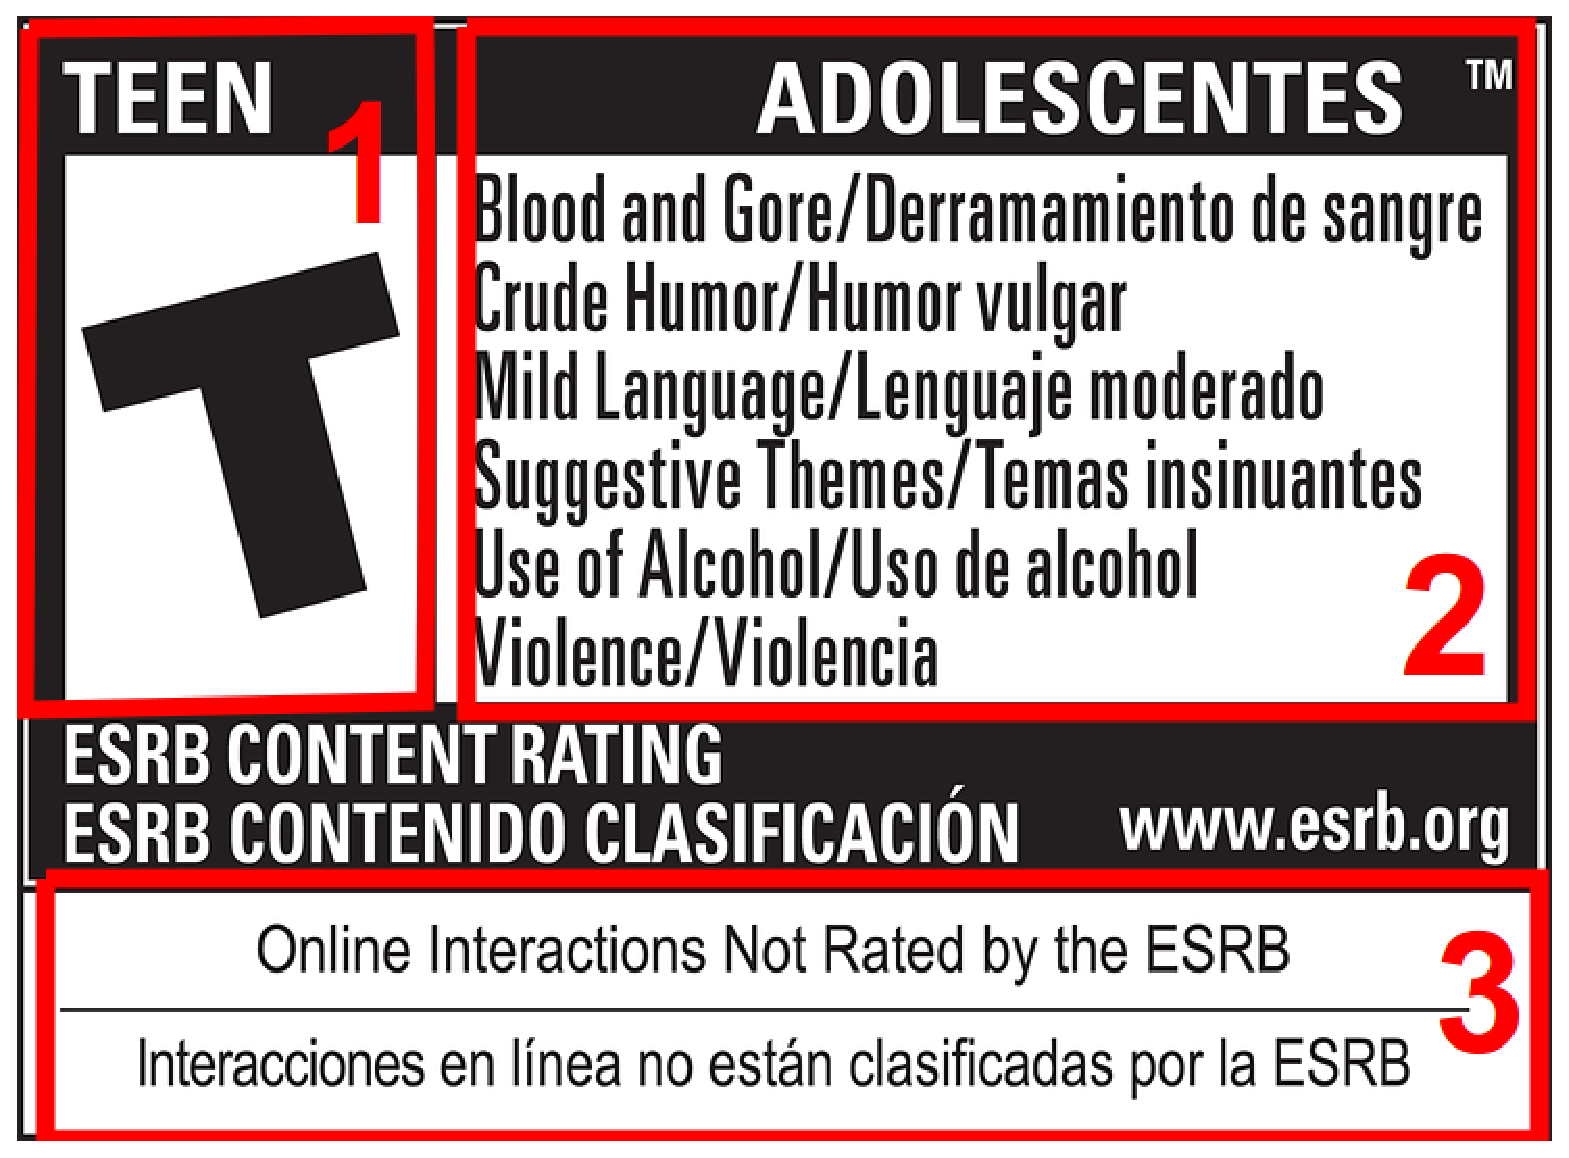
\includegraphics[width=0.4 \textwidth]{03MarcoTeoricoA/imagenes/etiqueta.eps}
					\caption{Etiqueta de clasificación de la ERSB. Esta compuesta de 
					tres partes: 1. Categorías de clasificación. 2. Descriptores de 
					contenido. 3. Elementos Interactivos $ [Imagen] (s/f)$ Recuperado 
					de: \url{http://media.blizzard.com/global-video-player/ratings-png/wow-cataclysm-esrb-esmx.png} } 
					\label{fig_etiquetaERSB}
		\end{figure}
		%,natwidth=737,natheight=540  ,natwidth=407,natheight=608
		\begin{figure}
					\centering
					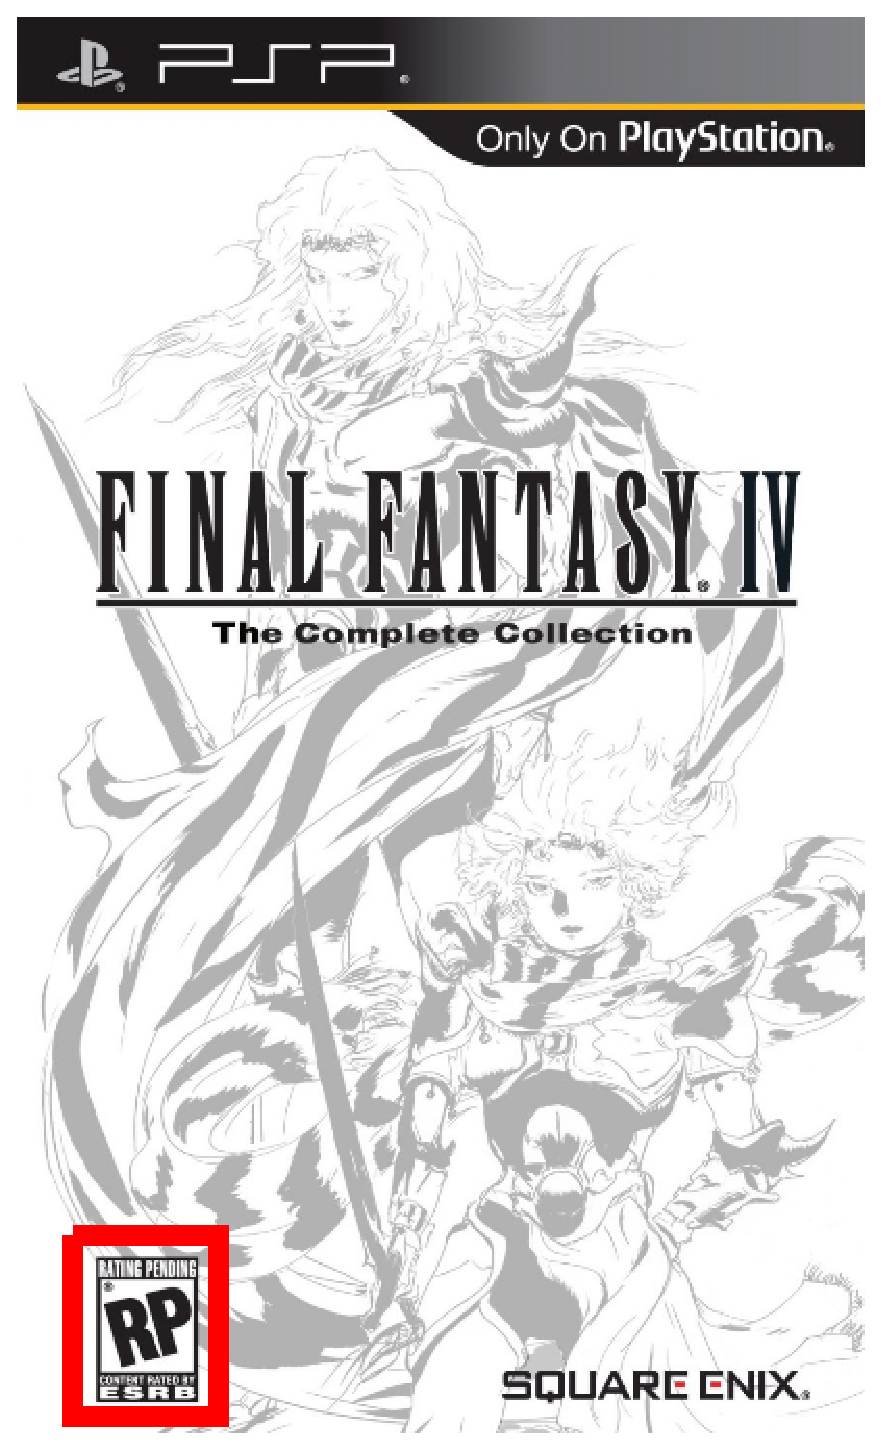
\includegraphics[width=0.3 \textwidth]{03MarcoTeoricoA/imagenes/FFCaratula.eps}
					\caption{Carátula de un juego con la etiqueta de clasificación ESRB 
					$[Imagen] (s/f)$ Recuperado de: \url{https://
					vignette.wikia.nocookie.net/es.finalfantasy/images/1/1c/
					FF4PSP\_NA\_Caratula.PNG/revision/latest?cb=20110301012441} } 
					\label{fig_caratulaERSB}
		\end{figure}
		\subsubsection{Clasificación por jugabilidad.}
		Esta clasificación es empleada por la industria para diferenciar los tipos de 
		juegos y de jugadores. A continuación se presenta la clasificación propuesta 
		en el libro "Juego. Historia, Teoría y Práctica del Diseño Conceptual de 
		Videojuegos"\cite{Ref_JuegoDisenio}  
			\begin{itemize}
			%===== Juegos de accion =====%
				\item \textbf{Juegos de acción:} Son juegos usualmente de temática 
				violenta. El jugador lucha por su supervivencia, para ello se vale 
				de armas o habilidades de  combate. Los juegos de acción se subdividen 
				en:
				\begin{itemize}
					\item \textbf{Juegos de lucha:} Este tipo de juego involucra lucha
					 cuerpo a cuerpo, con una fuerte infliuencia de las artes marciales.
					\item \textbf{Juegos de disparos:} Son aquellos en donde el jugador 
					mueve a su personaje para superar diversos escenarios en donde el 
					jugador debe de hacer uso de su armamento para lograr completar el 
					nivel.
					\item \textbf{Juego de plataformas:} El jugador debe de controlar a 
					un personaje con el que se dezplazará saltando entre plataformas y 
					esquivando todo tipo de obstáculos y enemigos.
				\end{itemize}
			%==== Juegos de estrategia ====%
				\item \textbf{Juegos de estrategia:} Para que el jugador logre sus 
				objetivos en este tipo de juegos, éste debe de planear una estrategia, 
				normalmente a lago plazo. La temática del juego de estrategia se 
				relaciona más con la escala y la visión. Lo juegos de estrategia 
				usualmente involucran mapas de gran tamaño, visión sobre el campo, 
				gestión de recursos, manejo de tropas, desarrollo de recursos, comercio 
				e intercambio de recursos, modificadores del campo, control de 
				territorio, etc.
			%==== Juegos de Rol ====%
				\item \textbf{Juegos de Rol:} Estos juegos tienen sus orígenes en los 
				juegos de rol de mesa. La mecánica de los juegos de rol gira en torno a 
				un grupo de héroes, con habilidades y progresión definidos; el grupo de 
				héroes debe de trabajar coordinadamente para cumplir un objetivo; estos 
				héroes pueden ser controlados por un solo jugador o por varios. El 
				jugador deberá explorar un mundo de gran tamaño haciendo evolucionar a 
				sus personajes y sus habilidades. En los juegos de rol, el uso y 
				recolección de objetos tiene un gran peso en la capacidad de avance del 
				jugador.
				\item \textbf{Videojuego de aventura:} Son parecidos a los juegos de 
				Rol; con la peculiaridad de que tienen una progresión más lineal y no 
				se hace tanto énfasis en los combates, siendo su eje principal la 
				narrativa.
				\item \textbf{Videojuegos de deportes:} Son todos aquellos videojuegos 
				que tratan sobre deportes que no involucren la conducción de un 
				vehículo. Pueden ser juegos sobre fútbol, fútbol americano, tenis, etc.
				\item \textbf{Videojuegos de carreras de vehículos:} Son todos aquellos 
				se centran en las carreras con todo tipo de vehículos, mayoritariamente 
				automóviles.
				\item \textbf{Videojuegos {\it puzzle:}} Este tipo de juego involucra 
				la resolución de un problema a partir de la utilización de una serie 
				limitada de recursos, por lo que si los recursos no se utilizan de la 
				manera correcta el problema no podrá ser solucionado.  
			\end{itemize}
			
	\subsection{Industria del videojuego.}\label{IndusVideo}
	El videojuego como producto para masas nace en 1972 con el videojuego de Pong 
	desarrollado por la empresa Atari, es así como nace las primeras maquinas 
	recreativas, ver figura \ref{fig_MaquinaAtari}. En sus inicios los videojuegos se caracterizaban por el uso de 
	pantallas estáticas, entornos bidimensionales y formas abstractas de juego
	\cite{perez2010analisis}. A la aparición de las maquinas recreativas le seguirían 
	las primeras consolas de mesa desarrolladas principalmente por Atari. 
	\\
	\par

	\begin{figure}
					\centering
					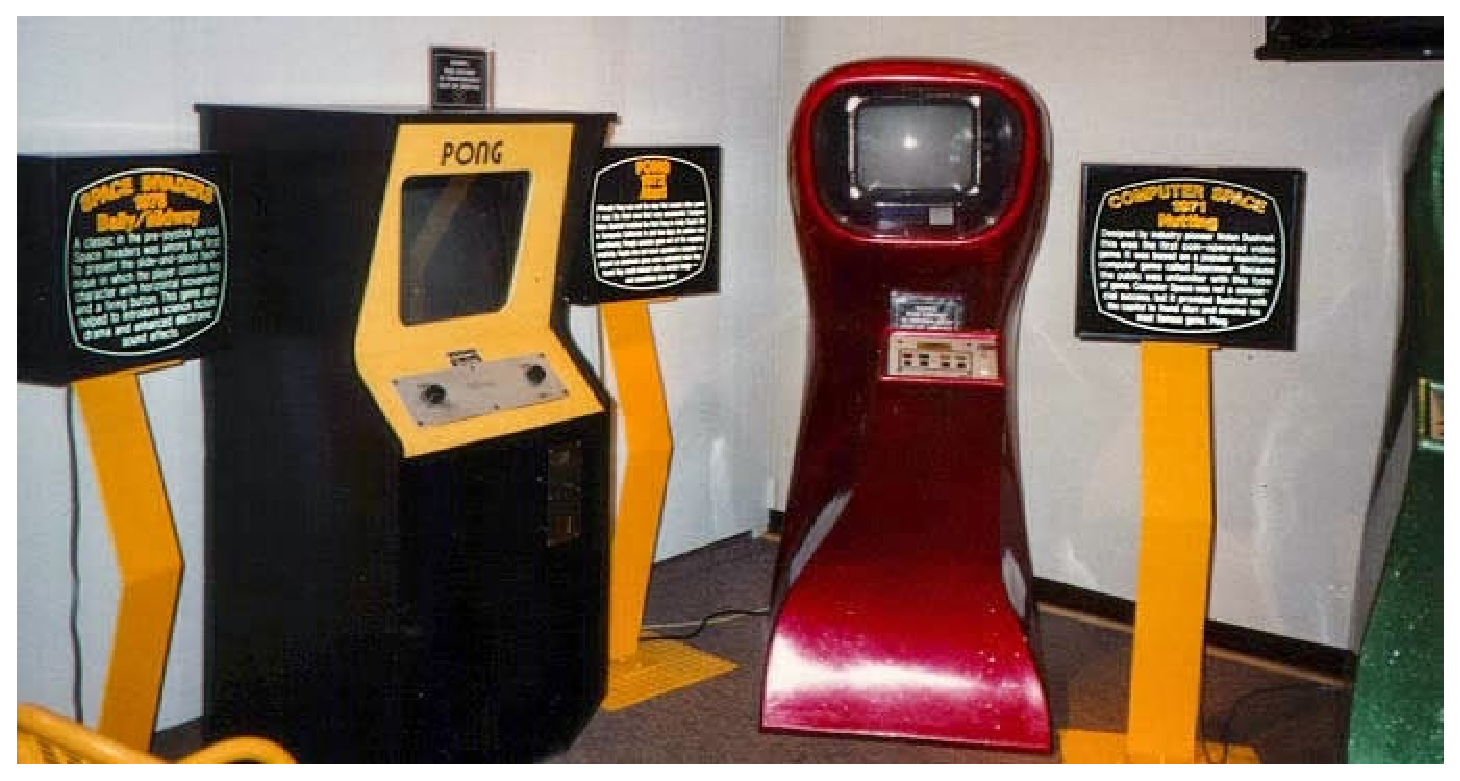
\includegraphics[width=0.5 \textwidth]{03MarcoTeoricoA/imagenes/atari.eps}
					\caption{Primeras maquinas recreativas desarrolladas por Atari 
					$[Imagen] (s/f)$ Recuperado de: \url{http://2.bp.blogspot.com/--98a06VymhA/VKJv2AQbNGI/AAAAAAAAAXU/rASZPNmBMrg/s1600/first\%2Barcades.jpg} } 
					\label{fig_MaquinaAtari}
		\end{figure}	
	
	Durante los años subsecuentes la industria del vidoejuego gozaría de una alta 
	tasa de recuperación; sin embargo la industria entraría en declive 1983, 
	empezando el periodo conocido como la crisis de los videojuegos, misma que 
	afectaría principalmente a las empresas estadounidenses y canadienses. Este 
	periodo duraría hasta 1985 y provocaría una polarización del mercado en donde 
	la industria japonesa de los videojuegos tomaría la ventaja frente a la 
	estadunidense. En 1983 la compañía Nintendo lanza al mercado su primera consola, 
	la Fumicom o Nintendo Entertainment System(NES) como fue conocida en el resto 
	del mundo \cite{belli2008breve}. Nintendo dio inicio a una nueva era para la 
	industria del videojuego con el lanzamiento de títulos que se consagraron como 
	clásicos de la industria y que al día de hoy aun se encuentran vigentes en el 
	mercado tales como Super Mario Bros, The Legend of Zelda, Pokemón, etc (ver figura \ref{fig:Nintendo}).
	\\	
	\par
	
	\begin{figure}
  		\centering
   		\subfigure[Super Mario Bros.] {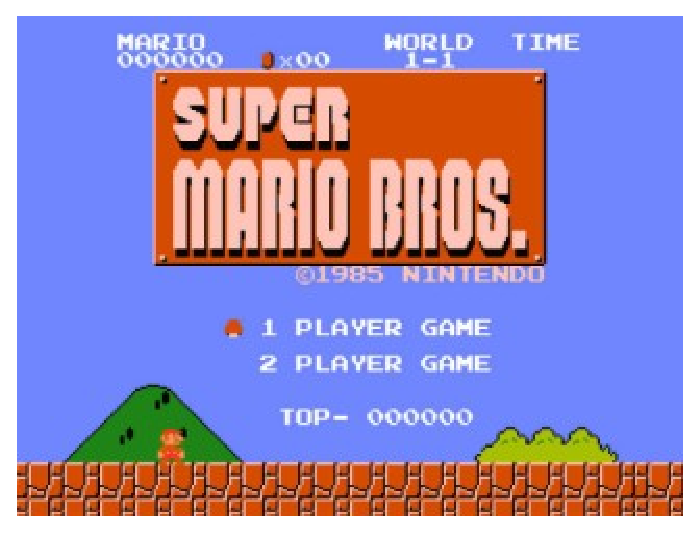
\includegraphics[width=0.3 				\textwidth]{03MarcoTeoricoA/imagenes/mario1.eps}}
   
 		\subfigure[The Legend of Zelda.]{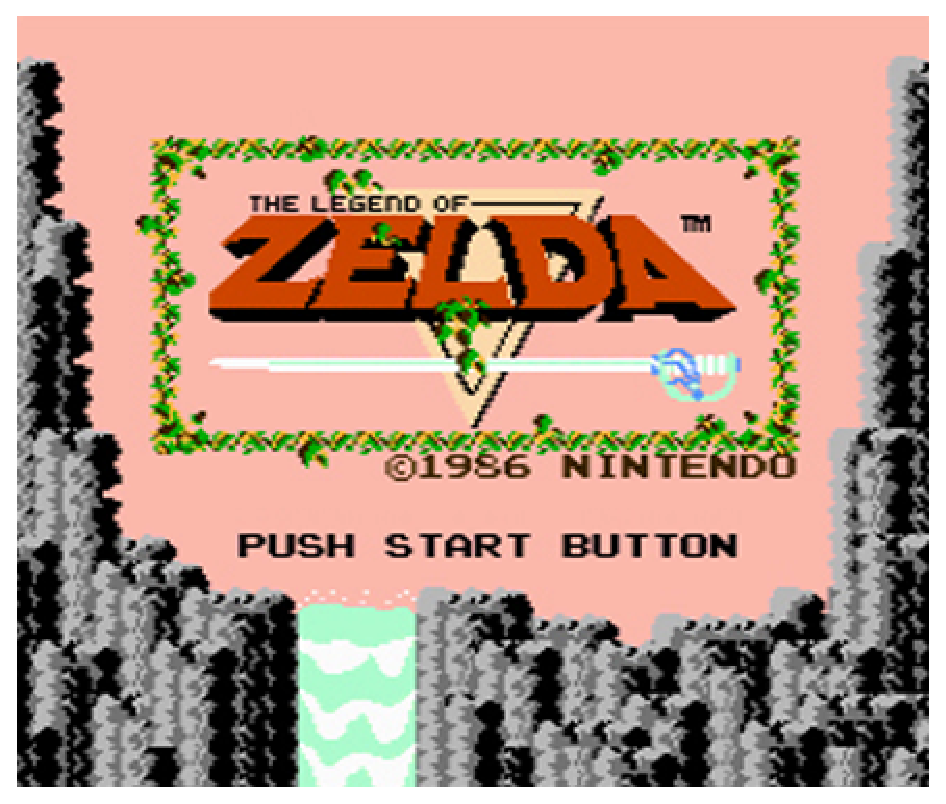
\includegraphics[width=0.3 \textwidth]{03MarcoTeoricoA/imagenes/zelda.eps}}
 	
		\subfigure[Pokemón.] {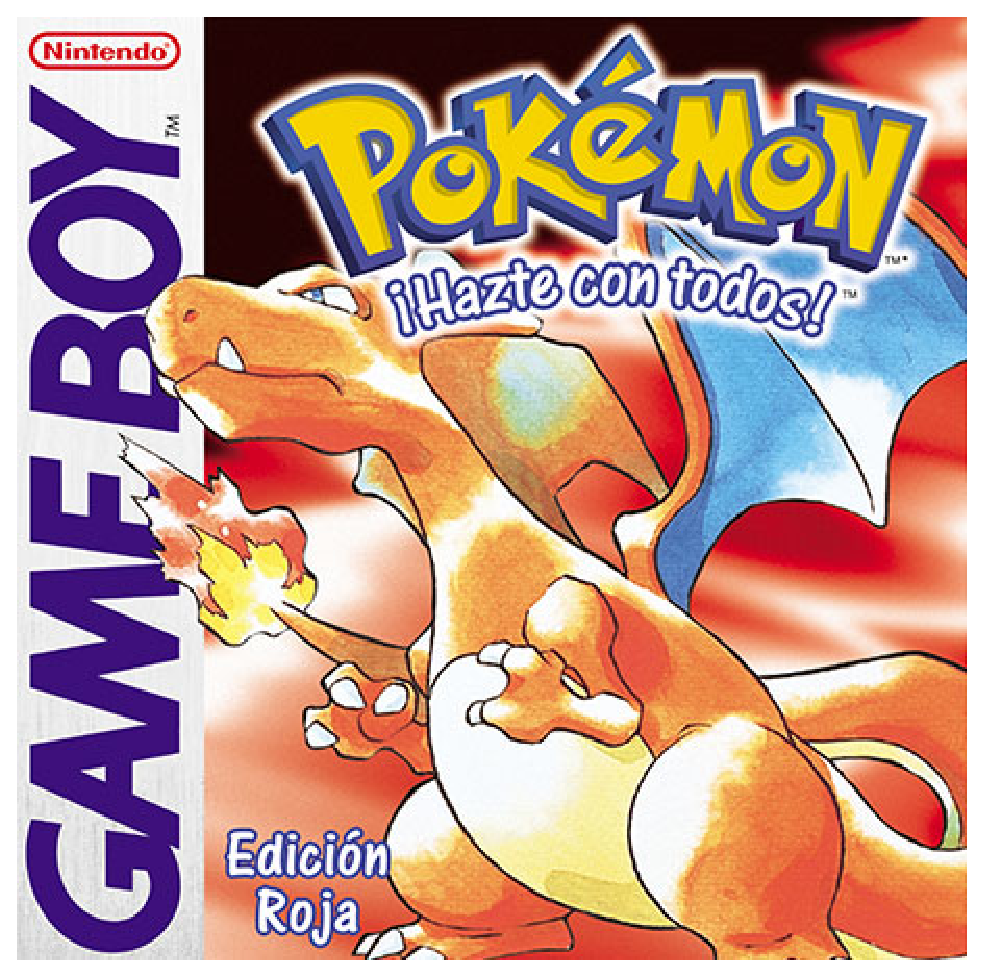
\includegraphics[width=0.3 \textwidth]{03MarcoTeoricoA/imagenes/pokemon.eps}}
  		\caption{Super Mario Bros, The Legend of Zelda y Pokemón son algunas de la franquicias más importantes de la compañía japonesa Nintendo.[Imagen] (s/f) Recuperado de (respectivamente): \url{http://contenidos.enter.co/custom/uploads/2015/09/mario1.jpg}, \url{https://www.hiddentriforce.com/wp-content/uploads/2015/02/10106454_5124592_lz.jpg}, \url{https://vignette.wikia.nocookie.net/es.pokemon/images/d/db/Car\%C3\%A1tula_de_Pok\%C3\%A9mon_Rojo.jpg}}
  		\label{fig:Nintendo}
	\end{figure} 

En las décadas posteriores, la industria del vidoejuego creció a un ritmo 
vertiginoso; no solo se diversifico el mercado con el nacimiento de nuevos 
géneros de videojuegos sino también las innovaciones tecnológicas de hardware 
permitieron crear cada vez mejores experiencias de juegos \cite{belli2008breve}. 
En menos de 20 años los videojuegos pasaron de entornos en dos dimensiones a 
entornos en tercera dimensión, del formato de almacenamiento en cartuchos al 
uso de CDs.	
	
Anualmente la induatria de los videojuegos genera miles de millones de dolares en ganancias, tan solo en el 2017 la industria generó 108.9 mil millones de dolares\cite{Ref_JuegosGanancia}. Estas ganancia fueron generadas un 25\% en Norteamerica, el 24\% en Europa, Medio Oriente y Africa, el 4\% en America latina, siendo la zona con mayor ingresos Asia y la zona del pacifico con el 47\% de ganancias generadas. En cuanto a la distribución de las ganacias con base a las plataformas, los telefonos moviles destronan a las consolas al generar el 32\% de las ganancias, mientras que las consolas han generado el 31\% de las ganancias, seguidas por las computadoras con el 23\%\cite{Ref_JuegosGanancia}.
	\\
	\par 
	%=== To do Poner las imagenes de las graficas de la estadistica
	
	\subsection{Industria del juego en México}
		La industria mexicana de videojuegos, al igual que la latinoamericana, es una industria emergente. Las empresas productoras de videojuegos mexicanas 
	\\
	\par
	México cerró el 2017 con un consumo de videojuegos de 1.4 mil millones de dolares, lo que le valio el doceavo puesto en cuanto a consumo de videojuegos a nivel mundial y el primer lugar en America latina. De acuerdo con los reportes de Unidad de Inteligencia Competitiva (CIU, por sus siglas en inglés) del 2016; en México hay 52.7 millones de jugadores, de los cuales el 71\% juega en dispositivos moviles\cite{Ref_IndusMEx}. Desafortunadamente y en contraposicion con estas cifras el consumo de videojuegos en México esta enforcado en juegos de origen extrangero. 
 